\documentclass[mat1]{fmfdelo}
% \documentclass[fin1]{fmfdelo}
% \documentclass[isrm1]{fmfdelo}
% \documentclass[mat2]{fmfdelo}
% \documentclass[fin2]{fmfdelo}
% \documentclass[isrm2]{fmfdelo}

% naslednje ukaze ustrezno napolnite
\avtor{Tom Gornik}

\naslov{Izrek o invarianci odprtih množic}
\title{Domain invariance theorem}

% navedite ime mentorja s polnim nazivom: doc.~dr.~Ime Priimek,
% izr.~prof.~dr.~Ime Priimek, prof.~dr.~Ime Priimek
% uporabite le tisti ukaz/ukaze, ki je/so za vas ustrezni
\mentor{ izr.~prof.~dr.~Jaka Smrekar}
% \mentorica{}
% \somentor{}
% \somentorica{}
% \mentorja{}{}
% \mentorici{}{}

\letnica{2020} % leto diplome

%  V povzetku na kratko opišite vsebinske rezultate dela. Sem ne sodi razlaga organizacije dela --
%  v katerem poglavju/razdelku je kaj, pač pa le opis vsebine.
\povzetek{}

%  Prevod slovenskega povzetka v angleščino.
\abstract{}

% navedite vsaj eno klasifikacijsko oznako --
% dostopne so na www.ams.org/mathscinet/msc/msc2010.html
\klasifikacija{}
\kljucnebesede{} % navedite nekaj ključnih pojmov, ki nastopajo v delu
\keywords{} % angleški prevod ključnih besed

\zapisiMetaPodatke  % poskrbi za metapodatke in veljaven PDF/A-1b standard

% aktivirajte pakete, ki jih potrebujete
\usepackage{tikz, verbatim, subcaption}
\usetikzlibrary{arrows.meta, calc, positioning, automata}

\newcommand{\literaturadiploma}{literaturadiploma}  % pot do datoteke z literaturo (brez .bib končnice)

\usepackage{bibentry}         % za navajanje literature v programu dela s celim imenom
%\nobibliography{\literaturadiploma}
\newcommand{\plancite}[1]{\item[\cite{#1}] \bibentry{#1}} % citiranje v programu dela


% za številske množice uporabite naslednje simbole
\newcommand{\R}{\mathbb R}
\newcommand{\N}{\mathbb N}
\newcommand{\Z}{\mathbb Z}
\newcommand{\C}{\mathbb C}
\newcommand{\Q}{\mathbb Q}
\newcommand{\I}{\mathbb I}
\newcommand{\0}{\underline{0}}
\newcommand{\Int}{\text{Int}}

% matematične operatorje deklarirajte kot take, da jih bo Latex pravilno stavil
% \DeclareMathOperator{\conv}{conv}

% vstavite svoje definicije ...
%  \newcommand{}{}

\begin{document}

\section{Izrek o invarianci odprtih množic}
V prejšnjih poglavjih smo si pripravili vse potrebno za dokaz izreka o invarianci odprtih množic, zato se bomo brez ovinkarjenja lotili dokaza.

\subsection{Navajanje literature}
Članke citiramo z uporabo \verb|\cite{label}|, \verb|\cite[text]{label}| ali pa več naenkrat s
\verb|\cite\{label1, label2}|. Tudi tukaj predhodno besedo in citat povežemo z nedeljivim presledkom
$\sim$. Na primer~\cite{chen2006meshless,liu2001point}, ali pa \cite{kibriya2007empirical}, ali pa
\cite[str.\ 12]{trobec2015parallel}, \cite[enačba (2.3)]{Schaefer2014}.
Vnosi iz \verb|.bib| datoteke, ki niso citirani, se ne prikažejo v seznamu literature, zato jih
tukaj citiram.~\cite{Engelking1989}, \cite{convexhull}, \cite{4dim},
\cite{Ahlbach}, \cite{Kulpa}, \cite{Gouvea2011}, \cite{simplex}. 

\begin{izrek}[Izrek o invarianci odprtih množic]\label{izr:main-theorem}
Naj bo $U \subset \R^n$ odprta podmnožica evklidskega prostora $\R^n$ in naj bo $h : U \rightarrow \R^n$ zvezna injektivna preslikava.
Potem je tudi slika $h(U)$ odprta množica v $\R^n$.
\end{izrek}

\begin{dokaz}
Naj bodo izpolnjene predpostavke izreka. Imamo množico U, ki je odprta podmnožica v $\R^n$ in zvezno injektivno preslikavo $h : U \rightarrow \R^n$. Izrek bo dokazan, če pokažemo, da je za vsak element $u$ iz množice $U$ točka $h(u)$ notranja točka za množico $h(U)$. Ker je $\R^n$ homogen prostor, take pa so tudi vse njegove odprte podmnožice, lahko predpostavimo, da je $u = 0_n$ in pokažemo, da je $h(0)$ notranja točka za $h(U)$. Izberimo tako pozitivno realno število $a > 0$, za katero je $\I^n \subset U$. Za dokaz izreka  je dovolj pokazati vsebovanost $b := h(0) \in \Int(h(\I^n))$. Od tu naprej bomo dokazovali s protislovjem. Privzeli bomo, da je $b \in \partial h(\I^n)$ in konstruirali funkcijo $f : \I^n \to \R^n \setminus \{ 0 \}$, tako da bo f zadoščala pogojem izreka~\ref{izr:PM}. To pa bo protislovje, saj mora taka funkcija po izreku~\ref{izrPM} vsaj eno točko slikati v $0$. Na poti do protislovja si bomo seveda pomagali tudi z lemami, ki smo jih spoznali in dokazali v prejšnjih poglavjih. Predpostavimo torej, da je $b \in \partial (\I^n)$. Ker je $\I^n$ kompaktna podmnožica $\R^n$ in je $\R^n$ houssdorfov prostor, je funkcija $h|_{\I^n} : \I^n \to \R^n$ homeomorfizem. Zato obstaja tako pozitivno realno število $\delta > 0$, za katerega je $h^{-1}(B(b, 2 \delta)) \subset \Int(\I^n)$. Ker je $b \in \partial h(\I^n)$ je mogoče poiskati tak $c \in B(b, \delta) \setminus h(I^n)$. Enostavno se je prepričati, da je $b \in B(c, \delta)$ in $h^{-1} (B(c, \delta)) \subset \Int (\I^n)$.

% ###############        Slika dokaza PM izreka ############
\begin{figure}[h!]
	\centering
	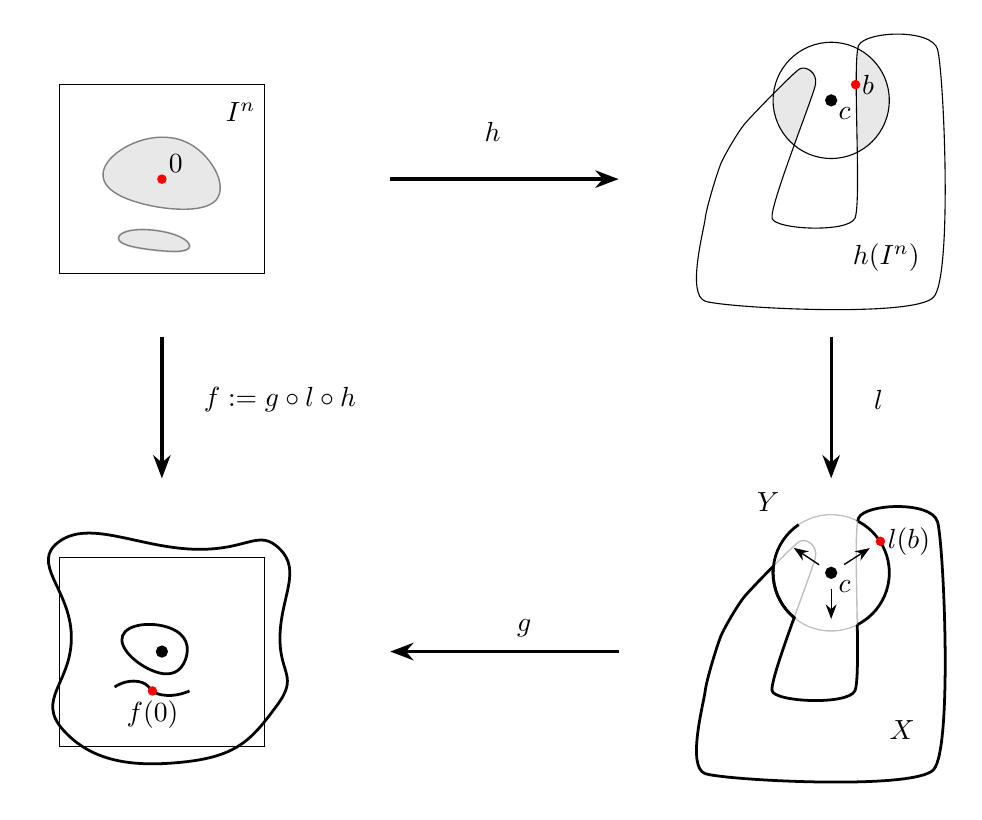
\begin{tikzpicture}
% ###############          prva slika          ###############
		\filldraw[color=gray!18] plot [smooth cycle, tension = 0.9] coordinates {(-5.15, 3.35) (-5.15, 2.8) (-3.95, 2.7) (-4.25, 3.45)};
		\draw[gray, line width=0.5pt] plot [smooth cycle, tension = 0.9] coordinates {(-5.15, 3.35) (-5.15, 2.8) (-3.95, 2.7) (-4.25, 3.45)};
		\filldraw[color=gray!18, line width=1pt] plot [smooth cycle, tension = 1.1] coordinates {(-4.25, 2.15) (-4.7, 2.35) (-5.15, 2.25) (-4.7, 2.1)};
		\draw[gray, line width=0.5pt] plot [smooth cycle, tension = 1.1] coordinates {(-4.25, 2.15) (-4.7, 2.35) (-5.15, 2.25) (-4.7, 2.1)};
		\draw (-5.9, 1.8) rectangle (-3.3, 4.2);
		\filldraw[red] (-4.6, 3) circle (1.5pt) node[black, above right=-0.5mm] {$0$};
		\draw (-4.2, 3.1) ;	
		 \draw (-3.6, 3.85) node {$I^n$};
		
% ###############          druga slika          ###############
		\begin{scope}
			\clip plot [smooth cycle, tension = 0.3] coordinates {(2.3, 1.45) (5.2, 1.5) (5.25, 4.65) (4.25, 4.7) (4.2, 2.5) (3.15, 2.5) (3.7, 4.2) (3.5, 4.4) (2.8,3.7)  (2.5, 3.2) (2.3, 2.5)};
			\clip (3.9, 4) circle (21pt);
			\fill[color=gray!18] (-2,1.5) rectangle (6,5);
		\end{scope}
		\draw plot [smooth cycle, tension = 0.3] coordinates {(2.3, 1.45) (5.2, 1.5) (5.25, 4.65) (4.25, 4.7) (4.2, 2.5) (3.15, 2.5) (3.7, 4.2) (3.5, 4.4) (2.8,3.7)  (2.5, 3.2) (2.3, 2.5)};
		\filldraw[black] (3.9, 4) circle (2pt) node[black, below right=-0.4mm]{$c$};
		\filldraw[red] (4.21, 4.2) circle (1.5pt) node[black, right=-0.4mm] {$b$};
		\draw[black] (3.9, 4) circle (21pt);
		\draw (4.6, 2) node {$h(I^n)$};
	
% ###############          tretja slika          ###############
		\draw[lightgray, line width=0.5pt] (3.9, -2) circle (21pt);
		\draw[black, line width=1pt] plot [smooth cycle, tension = 0.3] coordinates {(2.3, -4.55) (5.2, -4.5) (5.25, -1.35) (4.25, -1.3) (4.2, -3.5) (3.15, -3.5) (3.7, -1.8) (3.5, -1.6) (2.8, -2.3)  (2.5, -2.8) (2.3, -3.5)};
		\filldraw[white] (3.9, -2) circle (20.5pt);
		\begin{scope}
			\clip (3.9, -2) circle (21pt);
			\draw[lightgray, line width=0.5pt] plot [smooth cycle, tension = 0.3] coordinates {(2.3, -4.55) (5.2, -4.5) (5.25, -1.35) (4.25, -1.3) (4.2, -3.5) (3.15, -3.5) (3.7, -1.8) (3.5, -1.6) (2.8, -2.3)  (2.5, -2.8) (2.3, -3.5)};
		\end{scope}
		\begin{scope}
			\clip (3.9, -2) -- (3.4, -1.26) -- (2.5, -1) -- (3.35, -2.7) -- cycle;
			\draw[black, line width=1pt] (3.9, -2) circle (21pt);
		\end{scope}
		\begin{scope}
			\clip plot [smooth cycle, tension = 0.3] coordinates {(2.3, -4.55) (5.2, -4.5) (5.25, -1.35) (4.25, -1.3) (4.2, -3.5) (3.15, -3.5) (3.7, -1.8) (3.5, -1.6) (2.8, -2.3)  (2.5, -2.8) (2.3, -3.5)};
			\draw[black, line width=1pt] (3.9, -2) circle (21pt);
		\end{scope}
		\filldraw[black] (3.9, -2) circle (2pt) node[black, below right=-0.4mm]{$c$};
		\draw[black, line width=0.5pt, -Stealth] ($($(3.9, -2)!.5!(4.525, -1.6)$)!5pt!(3.9, -2)$) --  ($($(3.9, -2)!.5!(4.525, -1.6)$)!6pt!(4.525, -1.6)$);
		\draw[black, line width=0.5pt, -Stealth] ($($(3.9, -2)!.5!((3.9, -2.75)$)!5pt!(3.9, -2)$) --  ($($(3.9, -2)!.5!((3.9, -2.75)$)!6pt!((3.9, -2.75)$);
		\draw[black, line width=0.5pt, -Stealth] ($($(3.9, -2)!.5!(3.3, -1.6)$)!5pt!(3.9, -2)$) --  ($($(3.9, -2)!.5!(3.3, -1.6)$)!6pt!(3.3, -1.6)$);
		\filldraw[red] (4.525, -1.6) circle (1.5pt) node[black, right=-0.3mm] {$l(b)$};
		\draw (3.1, -1.1) node {$Y$};
		\draw (4.8, -4) node {$X$}; 
		
	% ###############          četrta slika          ###############
		\draw (-5.9, -4.2) rectangle (-3.3, -1.8);
		\draw[black, line width=1pt] plot [smooth cycle, tension = 1] coordinates {(-4.5, -2.7) (-4.3, -3.1) (-4.7, -3.25) (-5.1, -2.8)};
		\draw[black, line width=1pt] plot [smooth, tension = 1] coordinates {(-5.2, -3.45) (-4.9, -3.38) (-4.6, -3.55) (-4.25, -3.5)};
		\filldraw[red] (-4.72, -3.5) circle (1.5pt) node[black, below] {$f(0)$};
		\filldraw[black] (-4.6, -3) circle (2pt);
		\draw[black, line width=1pt] plot [smooth cycle, tension = 0.9] coordinates { (-3.1, -1.7) (-4.2, -1.7) (-5.9, -1.6) (-5.75, -2.8) (-5.85, -4) (-4.3, -4.4) (-3.15, -3.7) (-3.1, -2.8)};
	
	% ###############          puščice          ###############
		\draw [black, line width=1.2pt, -Stealth] (-1.7,3) -- (1.2,3);
		\draw (-0.4, 3.6) node {$h$};
		\draw [black,  line width=1.2pt, -Stealth] (1.2, -3) -- (-1.7, -3);
		\draw (0, -2.7) node {$g$};
		\draw [black,  line width=1.2pt, -Stealth] (-4.6, 1) -- (-4.6, -0.8);
		\draw (-3.1, 0.2) node {$f  := g \circ l \circ h$};
		\draw [black,  line width=1.2pt, -Stealth] (3.9, 1) -- (3.9, -0.8);
		\draw (4.5, 0.2) node {$l$};  
	\end{tikzpicture}
	\caption{Skica dokaza izreka~\ref{izr:main-theorem}.}
\end{figure}

Označimo $X := h(\I^n) \setminus B(c, \delta)$ in $Y := \partial B(c, \delta)$. Definiramo zvezno preslikavo $l : h(\I^n) \cup Y \to X \cup Y$ s predpisom:
\[  l(x) = \left\{
\begin{array}{ll}
	c + \frac{x - c}{\| x - c \|} \cdot \delta &, x \in h(\I^n) \cup B(c, \delta) \\
	x &, x \in X. \\
\end{array} 
\right. \]
S pomočjo leme~\ref{lem:razsiritev-nic} lahko preslikavo $h|_X : X \to \R^n \setminus \{ 0 \}$ razširimo do zvezne preslikave $g : X \cup Y \to \R^n \setminus \{ 0 \}$, za katero za vsak $x \in X$ velja $\| g(x) - h^{-1}(x) \| < a$.
Sedaj lahko definiramo preslikavo $f = (f_1, f_2, \dots, f_n) : \I^n \to \R \setminus \{ 0 \}$ kot kompozitum $f := g \circ l \circ h$. Ker ta funkcija slika iz $\I^n$ in ne zavzame ničle, je za protislovje dovolj, če se prepričamo, da funkcija ustreza pogojem izreka~\ref{izr:PM}. Vzemimo $t \in \I_i^-$. Velja $l(h(t)) = h(t)$, saj je $h(t) \in X$. Poglejmo normo $\| f(t) - t \| = \| g(l(h(t))) - h{-1}(h(t)) \| = \| g(h(t) - h{-1}(h(t)) \| < a$. Ker je $t_i = - a$ je $| f_i (t) - t_i | = | f_i (t) - ( - a) | \leq | f (t) - t | < a$ torej je $f_i(t) < 0$. Enako lahko sklepamo tudi v primeru, ko je $t_i \in \I_i^+$. Ugotovili smo, da je  $f_i(\I_i^-) < 0$ in $f_i(\I_i^+) > 0$, zato bi po predpostavkah izreka~\ref{izr:PM} moral obstajati $x \in \I^n$, ki se z $f$ slika v $0$. To je protislovje, torej je $b \in \Int (h(\I^n)$ in je $h(U)$ odprta podmnožica v $\R^n$.
\end{dokaz}

\begin{izrek}[Izrek o invarianci dimenzije]\label{izr:dim_izr}
Naj bosta $m$ in $n$ naravni števili, potem sta Evklidska prostora $\R^m$ in $\R^n$ homeomorfna, če in samo če je $m = n$.
\end{izrek}

\begin{dokaz}
Denimo, da sta za neki dve naravni števili $m$ in $n$ Evklidska prostora $\R^m$ in $\R^n$ homeomorfna. Torej obstaja zvezna bijektivna preslikava $f : \R^n \to \R^m$ z zveznim inverzom $f^{-1} : \R^m \to \R^n$. Dokazovali bomo s protislovjem. Predpostavimo, da je $m \neq n$, brez izgube splošnosti lahko predpostavimo , da je $m < n$. Označimo z $i$ vložitev, torej preslikavo iz prostora $\R^m$ v $\R^n$, ki je definirana s predpisom $i(x_1, \dots, x_m) = (x_1, \dots, x_m, 0, \dots, 0)$. Tedaj je preslikava $h : \R^n \to \R^n$ definirana kot kompozitum $h := i \circ f$ zvezna injektivna preslikava, zato je po izreku~\ref{izr:main-theorem} odprta. Toda slika prostora $\R^n$, ki je odprta podmnožica same sebe, je množica $\left \{ (x_1, x_2, \dots, x_m, 0, \dots, 0) \in \R^n ; \text{ kjer so } x_i \in \R \text{ za vsak } i \in \{1, \dots, m \}  \right \}$, ki pa je zaprta podmnožica prostora $\R^n$. Torej mora biti res $m = n$.
\end{dokaz}

% seznam uporabljene literature

\cleardoublepage                           % na desni strani
\phantomsection                            % da prav delujejo hiperlinki
\addcontentsline{toc}{section}{\bibname}   % dodajmo v kazalo
\bibliographystyle{fmf-sl}                 % uporabljen stil je v datoteki fmf-sl.bst, na voljo tudi angleška verzija
\bibliography{\literaturadiploma}        

\end{document}

